\documentclass[11pt]{article}
\usepackage[margin=0.8in]{geometry}
\usepackage{graphicx}
\usepackage{booktabs}
\usepackage{float}
\usepackage{adjustbox}
\usepackage{amsmath}
\usepackage{lmodern}
\usepackage[T1]{fontenc}
\IfFileExists{pdflscape.sty}{\usepackage{pdflscape}}{\usepackage{lscape}}
\usepackage{hyperref}
\graphicspath{{figures/}}

\title{Corporate Events and Business Positioning, Controlling for Item 1 Length}
\author{}
\date{\today}

\begin{document}
\maketitle

\noindent Business positioning is measured by $n_{\mathrm{parent}}$, the number of distinct parent
activities a firm reports in year $t$. Parent flows are \emph{parents entering} (parents in $t$ not
in $t-1$) and \emph{parents exiting} (parents in $t-1$ not in $t$); flows are missing in a firm's
first observed year and when year $t-1$ is not observed. Enter and exit shares divide the flow by
$n_{\mathrm{parent}}$ in $t$. The difference-in-differences and event-study regressions add $\ln(\text{Item 1 words})$ as a control, since
longer business descriptions mechanically list more activities. This control is used in the
difference-in-differences and event-study sections; the descriptive figures and the final
section (uniqueness and financial performance) do not use it.

\section{Descriptive Evidence}

Figure~\ref{fig:desc} plots the raw average of $n_{\mathrm{parent}}$ for treated firms in event
time $-6$ to $+6$ around each event. Event time $0$ is the event year. No controls or fixed
effects are applied (these figures do not use the Item 1 control).

\begin{figure}[H]
\centering
\begin{minipage}{0.32\textwidth}\centering
  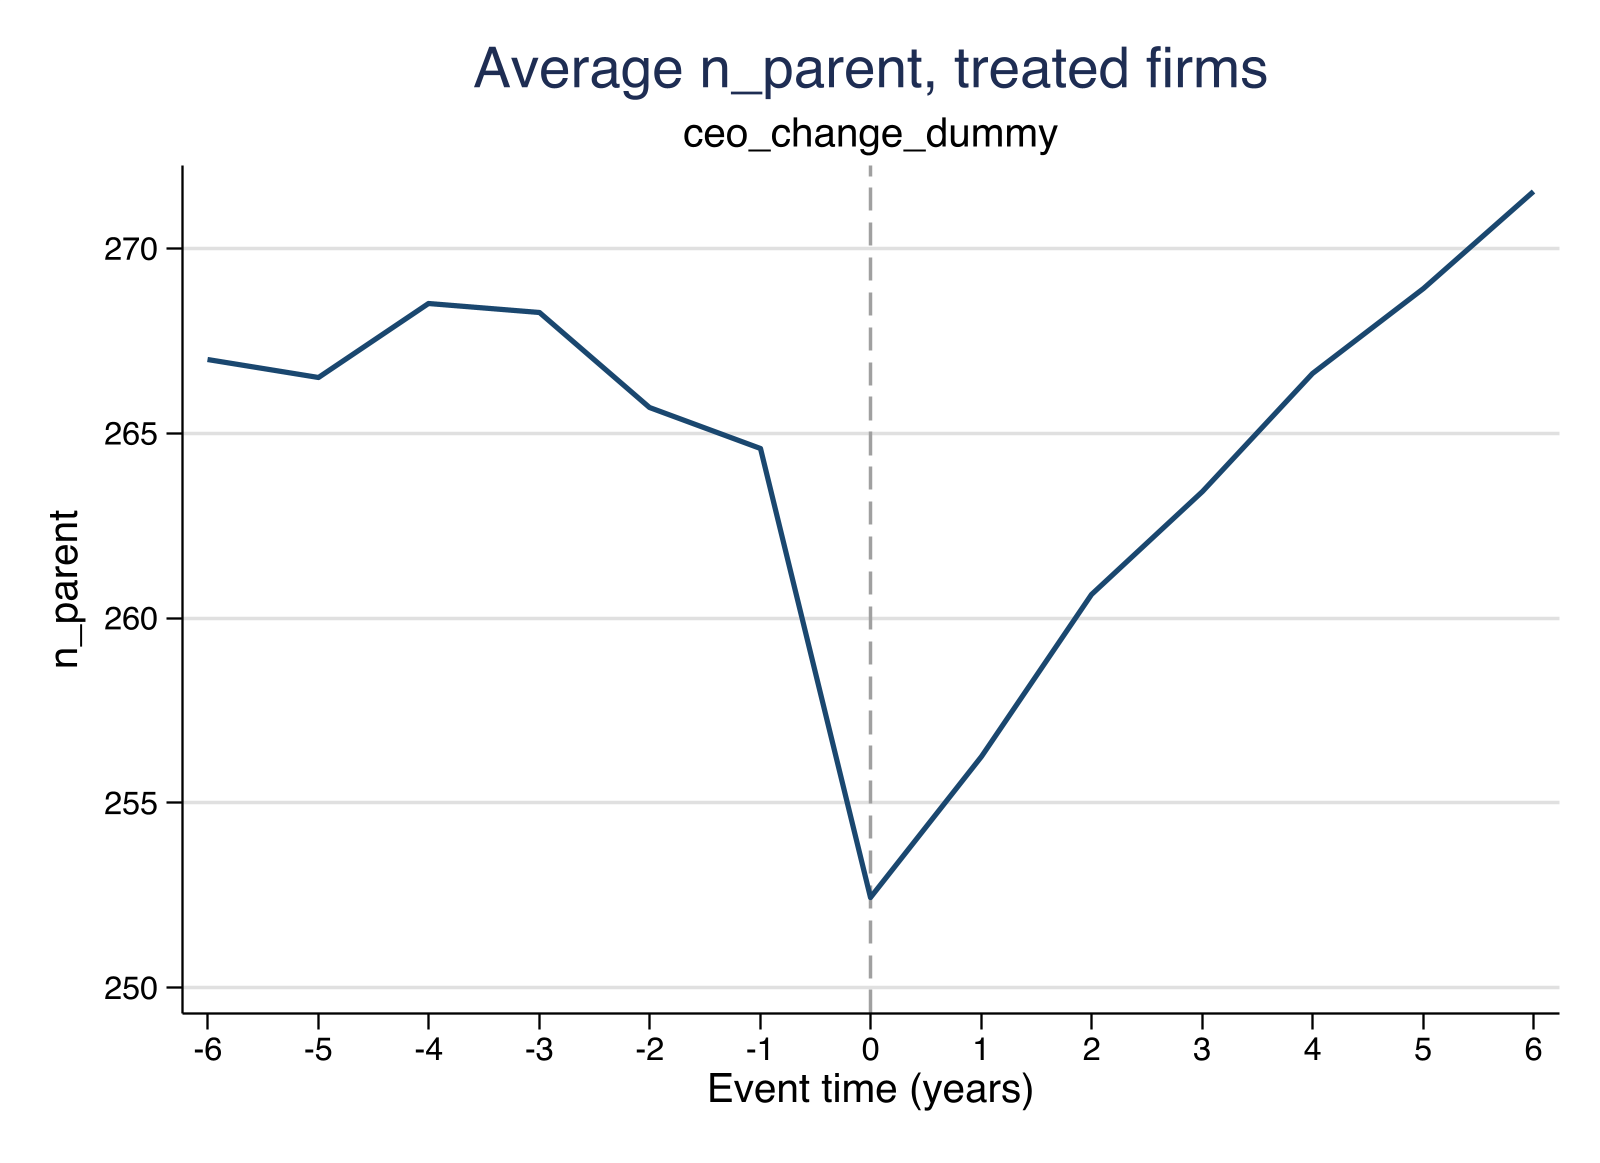
\includegraphics[width=\linewidth]{descriptive/mean_n_parent_ceo_change_dummy_treated.png}
  {\small (a) CEO Change}
\end{minipage}\hfill
\begin{minipage}{0.32\textwidth}\centering
  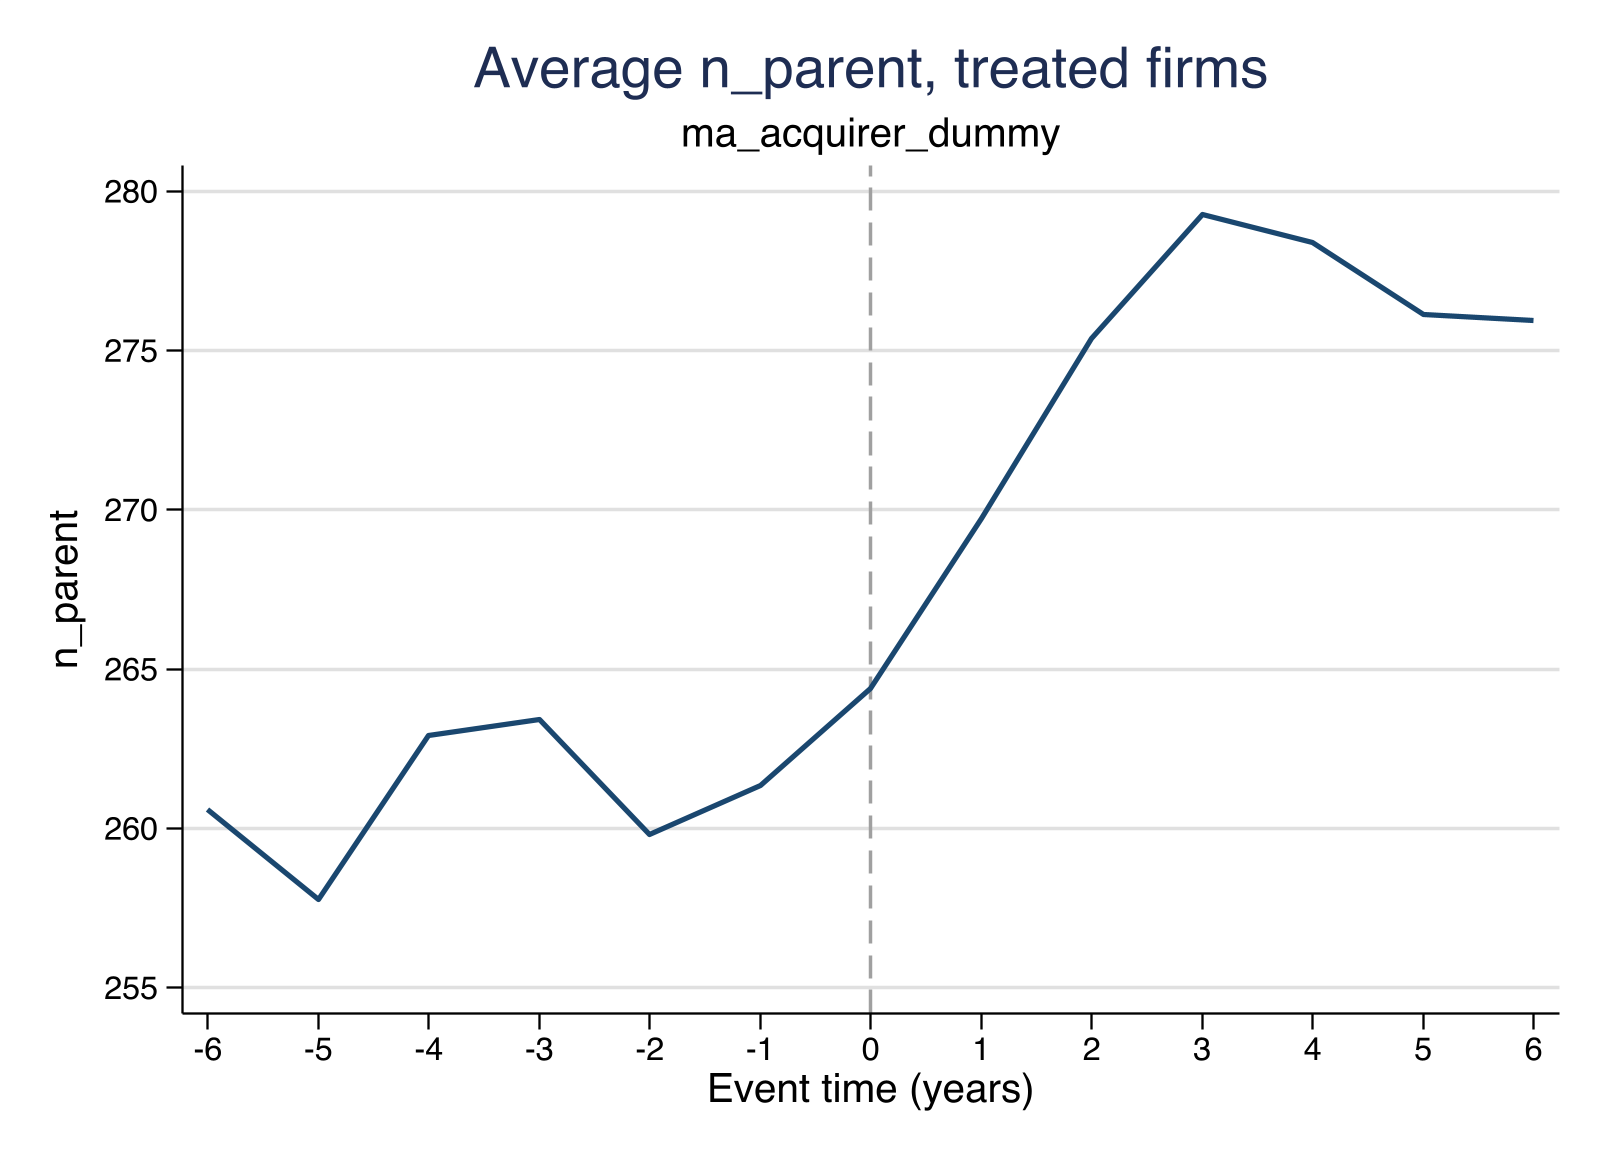
\includegraphics[width=\linewidth]{descriptive/mean_n_parent_ma_acquirer_dummy_treated.png}
  {\small (b) M\&A Acquirer}
\end{minipage}\hfill
\begin{minipage}{0.32\textwidth}\centering
  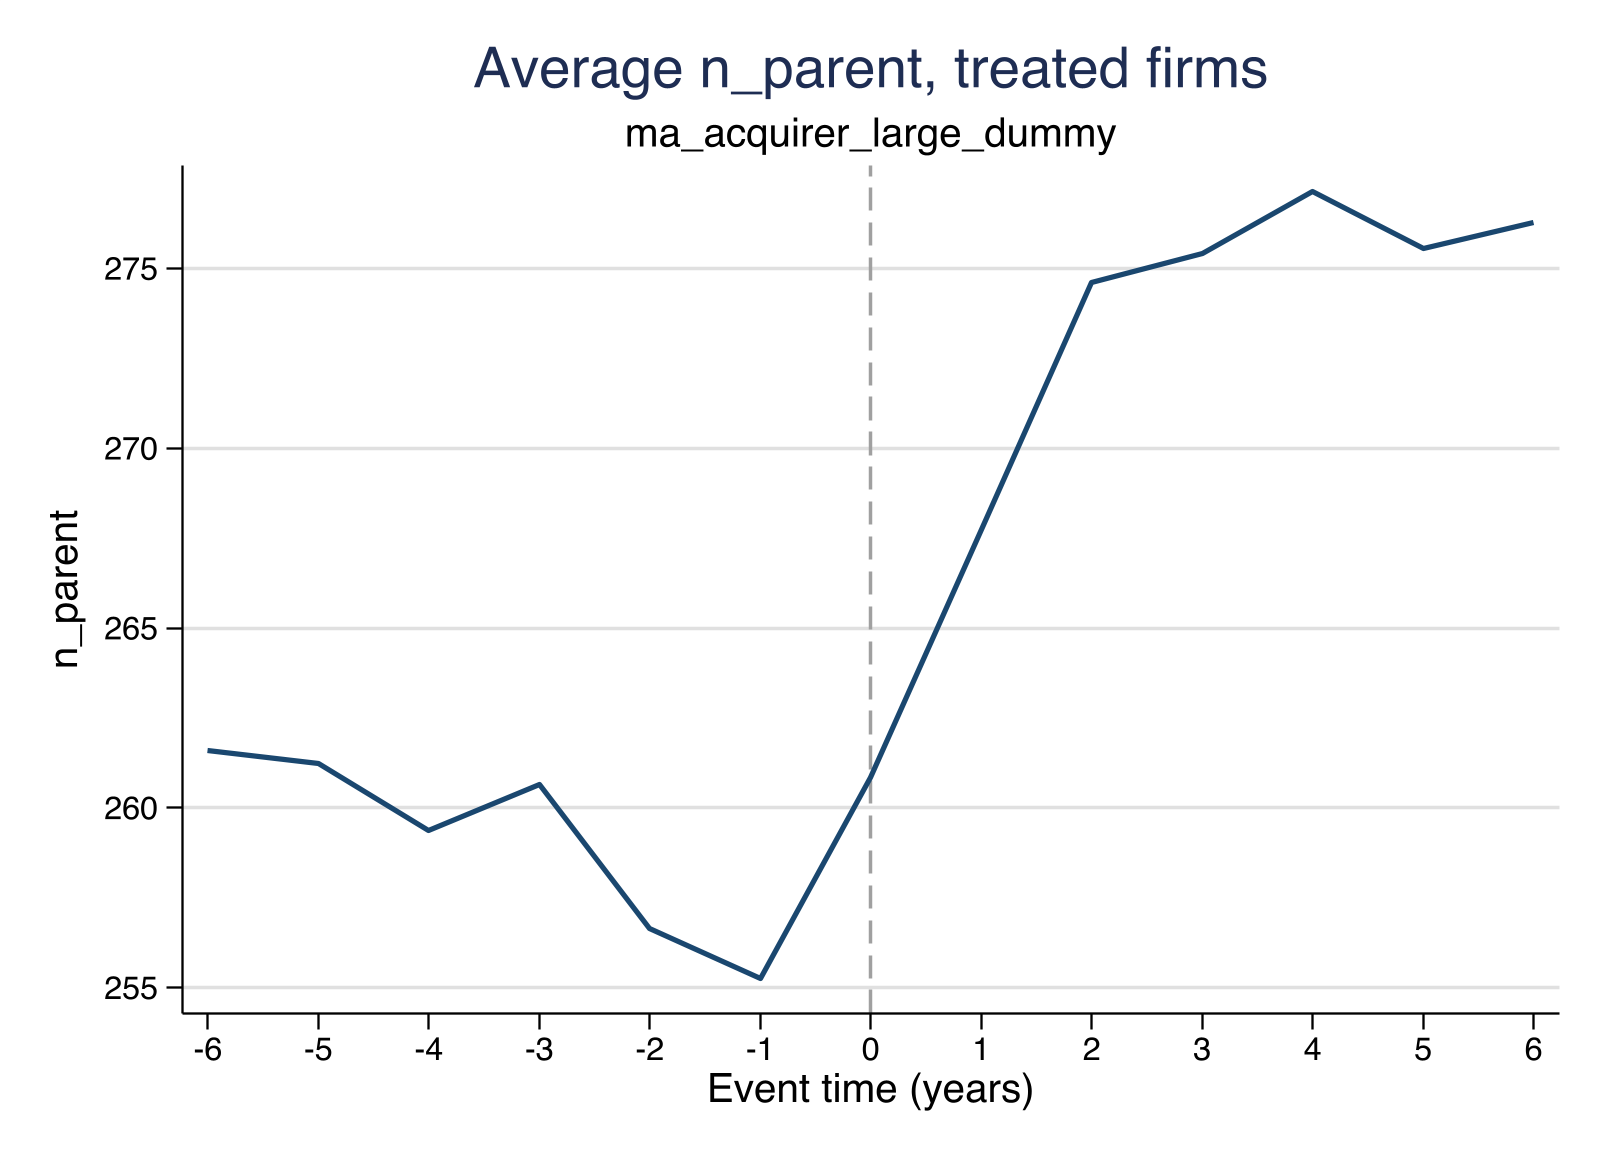
\includegraphics[width=\linewidth]{descriptive/mean_n_parent_ma_acquirer_large_dummy_treated.png}
  {\small (c) Large M\&A Acquirer}
\end{minipage}

\vspace{6pt}
\begin{minipage}{0.32\textwidth}\centering
  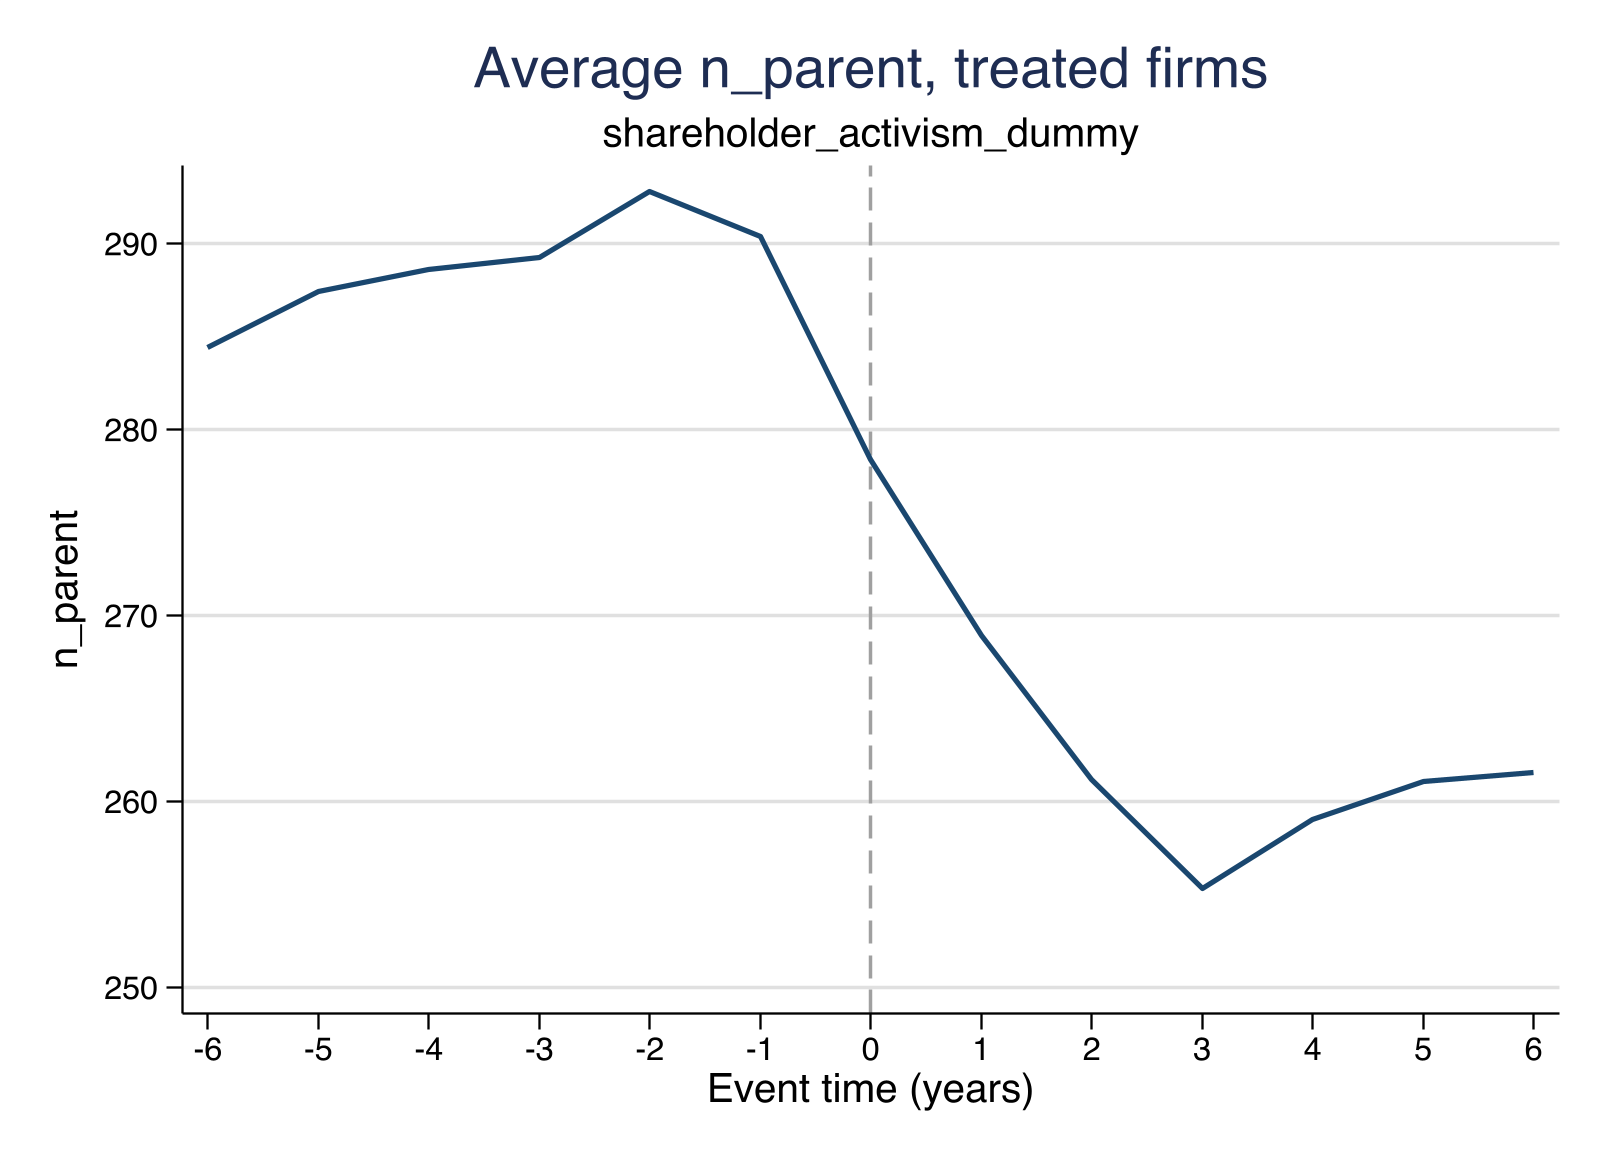
\includegraphics[width=\linewidth]{descriptive/mean_n_parent_shareholder_activism_dummy_treated.png}
  {\small (d) Shareholder Activism}
\end{minipage}\hfill
\begin{minipage}{0.32\textwidth}\centering
  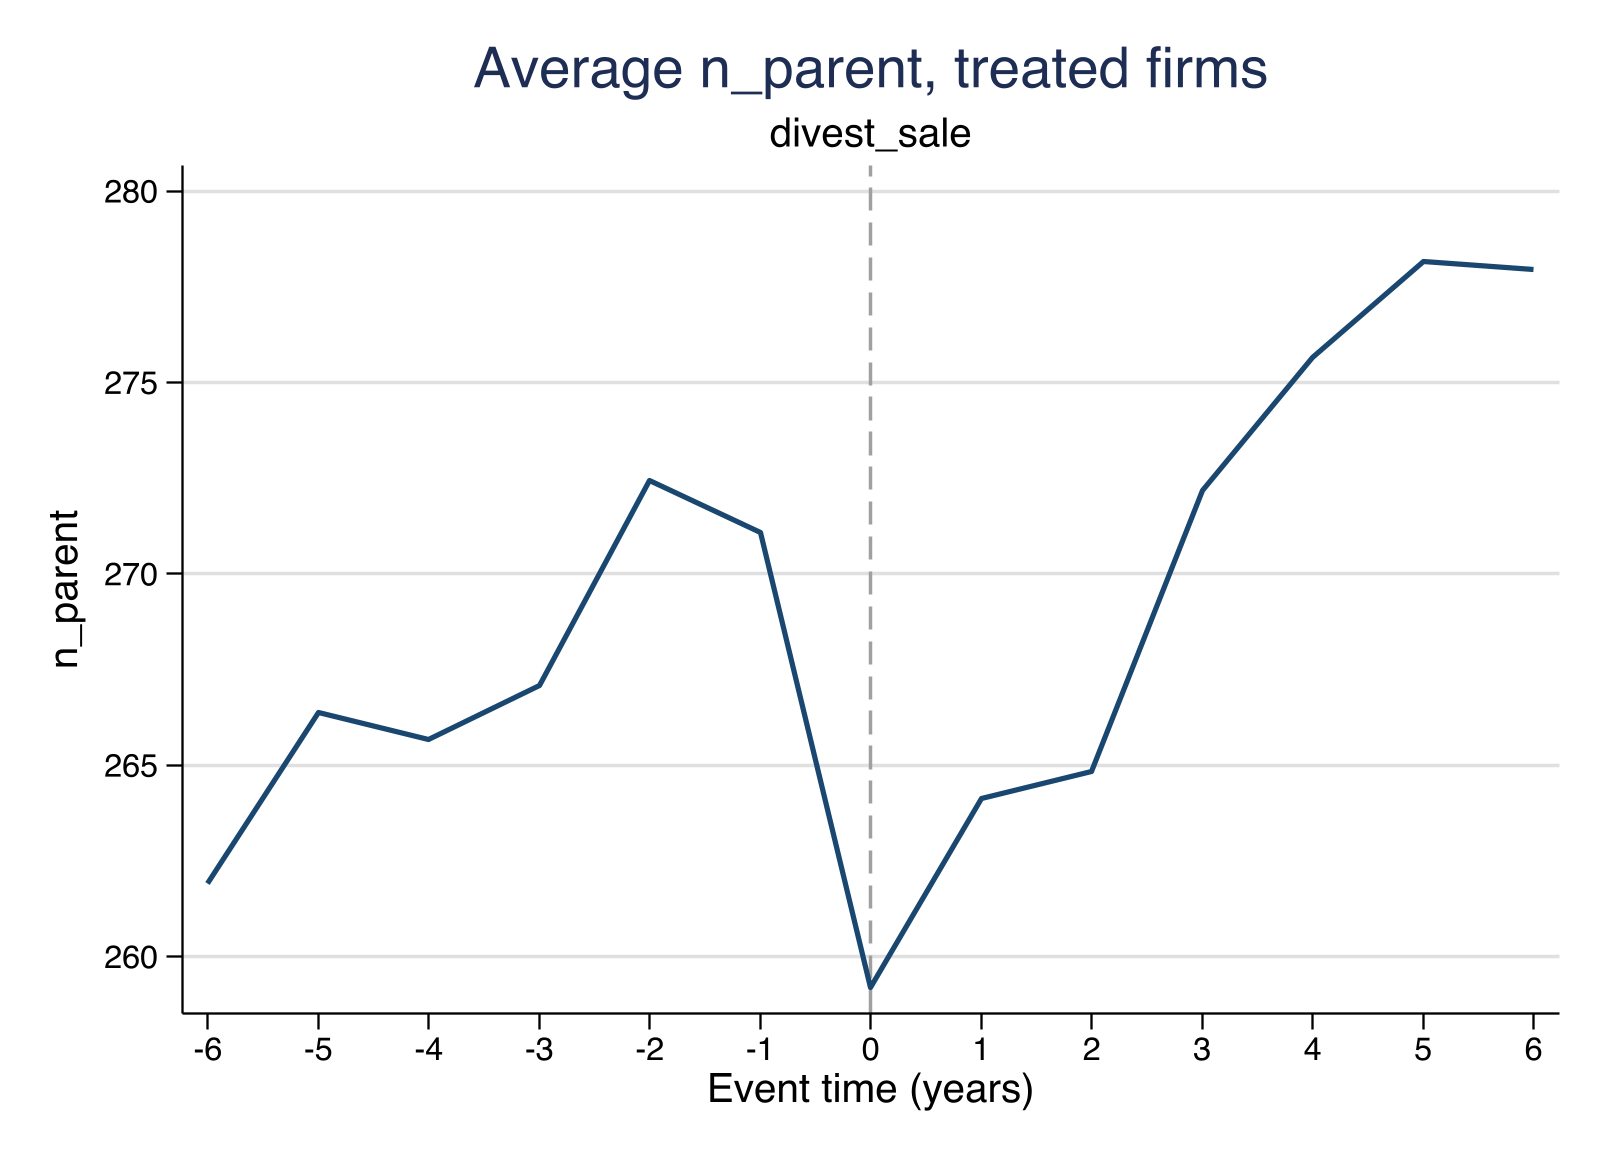
\includegraphics[width=\linewidth]{descriptive/mean_n_parent_divest_sale_treated.png}
  {\small (e) Divestiture}
\end{minipage}\hfill
\begin{minipage}{0.32\textwidth}\centering
  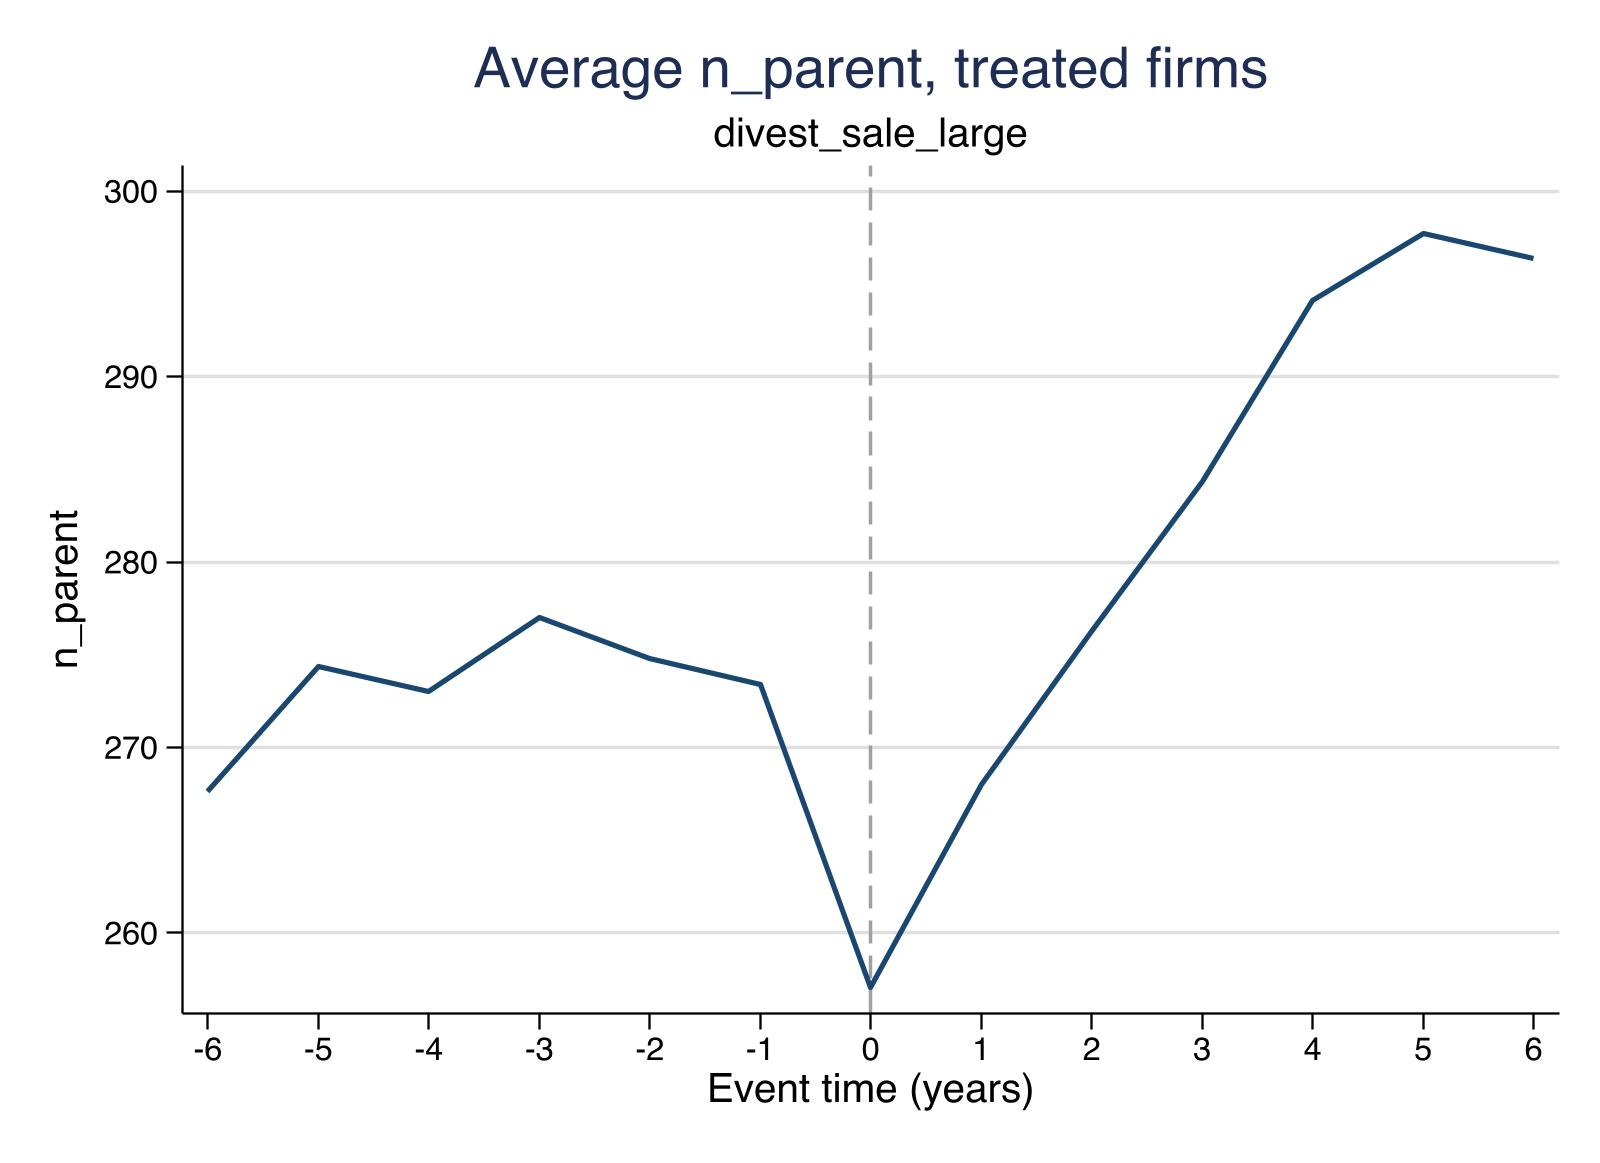
\includegraphics[width=\linewidth]{descriptive/mean_n_parent_divest_sale_large_treated.png}
  {\small (f) Large Divestiture}
\end{minipage}
\caption{Average $n_{\mathrm{parent}}$ of treated firms around the event (raw means).}
\label{fig:desc}
\end{figure}

\section{Corporate Events: Stacked Pre/Post Difference-in-Differences}

For every event (cohort) $c$ of firm $i$ we build a window from $-3$ to $+3$ years around the
event year, bounded by the firm's neighbouring events, and stack the cohorts. Control firm-years
come from firms that never experience the event, matched to each cohort by calendar year.
Each cell of Table~\ref{tab:did_item1} is a separate regression; for every event the first column
includes the Item 1 control and the second omits it:
\[
  y_{ict} = \beta \, \mathrm{Post}_{ict} \times \mathrm{Treated}_{ic} + \delta \ln(\text{Item 1 words}_{ict}) + \alpha_{ic} + \gamma_{tc} + \varepsilon_{ict},
\]
with firm $\times$ cohort and year $\times$ cohort fixed effects and standard errors clustered by firm.

\begin{landscape}
\begin{table}[H]
\centering
\caption{Stacked Pre/Post Difference-in-Differences Estimates}
\label{tab:did_item1}
{\small Event window: $-3$ to $+3$ years; with and without the $\ln$(Item 1 words) control}\\[4pt]
\begin{adjustbox}{max width=\linewidth, max totalheight=0.62\textheight}
\begin{tabular}{lcccccccc}
\toprule
 & \multicolumn{2}{c}{CEO Change} & \multicolumn{2}{c}{Large M\&A Acquirer} & \multicolumn{2}{c}{Shareholder Activism} & \multicolumn{2}{c}{Divestiture} \\
\cmidrule(lr){2-3} \cmidrule(lr){4-5} \cmidrule(lr){6-7} \cmidrule(lr){8-9}
 & (1) & (2) & (3) & (4) & (5) & (6) & (7) & (8) \\
\midrule
\multicolumn{9}{l}{\textit{Panel A. Dependent variable: $n_{\mathrm{parent}}$}} \\[2pt]
Post $\times$ treated & $-$5.670$^{**}$ & $-$5.747$^{**}$ & 3.765$^{**}$ & 8.464$^{***}$ & $-$11.927$^{***}$ & $-$13.765$^{***}$ & $-$5.403$^{**}$ & $-$5.974$^{**}$ \\
 & (1.765) & (2.060) & (1.293) & (1.539) & (2.108) & (2.638) & (1.704) & (2.058) \\
Pre-event treated mean & 262.746 & 262.746 & 259.688 & 259.688 & 285.331 & 285.331 & 268.739 & 268.739 \\
Observations & 51,003 & 51,003 & 98,127 & 98,127 & 173,667 & 173,667 & 178,953 & 178,953 \\
Treated event-year observations & 4,423 & 4,423 & 3,141 & 3,141 & 887 & 887 & 1,262 & 1,262 \\
Within $R^2$ & 0.2583 & 0.0011 & 0.2643 & 0.0014 & 0.2657 & 0.0005 & 0.2607 & 0.0002 \\
\cmidrule(l){1-9}
\addlinespace[4pt]
\multicolumn{9}{l}{\textit{Panel B. Dependent variable: Parents entering}} \\[2pt]
Post $\times$ treated & 2.768$^{***}$ & 2.686$^{***}$ & 5.976$^{***}$ & 7.373$^{***}$ & $-$2.746$^{**}$ & $-$3.455$^{***}$ & $-$0.144 & $-$0.265 \\
 & (0.704) & (0.786) & (0.586) & (0.648) & (0.986) & (1.033) & (0.827) & (0.883) \\
Pre-event treated mean & 45.878 & 45.878 & 46.198 & 46.198 & 48.208 & 48.208 & 50.396 & 50.396 \\
Observations & 45,736 & 45,736 & 89,023 & 89,023 & 163,129 & 163,129 & 164,020 & 164,020 \\
Treated event-year observations & 3,973 & 3,973 & 2,851 & 2,851 & 862 & 862 & 1,187 & 1,187 \\
Within $R^2$ & 0.0493 & 0.0005 & 0.0550 & 0.0024 & 0.0490 & 0.0001 & 0.0476 & 0.0000 \\
\cmidrule(l){1-9}
\addlinespace[4pt]
\multicolumn{9}{l}{\textit{Panel C. Dependent variable: Parents exiting}} \\[2pt]
Post $\times$ treated & 1.411 & 1.451 & 3.731$^{***}$ & 3.091$^{***}$ & 1.823 & 2.133 & $-$0.550 & $-$0.492 \\
 & (0.806) & (0.770) & (0.691) & (0.658) & (1.412) & (1.399) & (0.949) & (0.906) \\
Pre-event treated mean & 42.294 & 42.294 & 42.871 & 42.871 & 46.177 & 46.177 & 47.011 & 47.011 \\
Observations & 45,736 & 45,736 & 89,023 & 89,023 & 163,129 & 163,129 & 164,020 & 164,020 \\
Treated event-year observations & 3,973 & 3,973 & 2,851 & 2,851 & 862 & 862 & 1,187 & 1,187 \\
Within $R^2$ & 0.0096 & 0.0001 & 0.0093 & 0.0003 & 0.0079 & 0.0000 & 0.0093 & 0.0000 \\
\cmidrule(l){1-9}
\addlinespace[4pt]
\multicolumn{9}{l}{\textit{Panel D. Dependent variable: Enter share (enter / $n_{\mathrm{parent}}$)}} \\[2pt]
Post $\times$ treated & 0.0118$^{***}$ & 0.0117$^{***}$ & 0.0182$^{***}$ & 0.0206$^{***}$ & $-$0.0022 & $-$0.0033 & 0.0001 & $-$0.0001 \\
 & (0.0028) & (0.0028) & (0.0024) & (0.0024) & (0.0041) & (0.0041) & (0.0032) & (0.0032) \\
Pre-event treated mean & 0.1847 & 0.1847 & 0.1864 & 0.1864 & 0.1806 & 0.1806 & 0.1963 & 0.1963 \\
Observations & 45,736 & 45,736 & 89,023 & 89,023 & 163,129 & 163,129 & 164,020 & 164,020 \\
Treated event-year observations & 3,973 & 3,973 & 2,851 & 2,851 & 862 & 862 & 1,187 & 1,187 \\
Within $R^2$ & 0.0079 & 0.0007 & 0.0110 & 0.0012 & 0.0080 & 0.0000 & 0.0082 & 0.0000 \\
\cmidrule(l){1-9}
\addlinespace[4pt]
\multicolumn{9}{l}{\textit{Panel E. Dependent variable: Exit share (exit / $n_{\mathrm{parent}}$)}} \\[2pt]
Post $\times$ treated & 0.0058 & 0.0064 & 0.0246$^{**}$ & 0.0102 & 0.0308$^{**}$ & 0.0373$^{***}$ & $-$0.0053 & $-$0.0042 \\
 & (0.0090) & (0.0089) & (0.0087) & (0.0080) & (0.0110) & (0.0112) & (0.0083) & (0.0079) \\
Pre-event treated mean & 0.1954 & 0.1954 & 0.1913 & 0.1913 & 0.1884 & 0.1884 & 0.2112 & 0.2112 \\
Observations & 45,736 & 45,736 & 89,023 & 89,023 & 163,129 & 163,129 & 164,020 & 164,020 \\
Treated event-year observations & 3,973 & 3,973 & 2,851 & 2,851 & 862 & 862 & 1,187 & 1,187 \\
Within $R^2$ & 0.0240 & 0.0000 & 0.0336 & 0.0000 & 0.0277 & 0.0001 & 0.0223 & 0.0000 \\
\midrule
Item 1 Words Control & Yes & No & Yes & No & Yes & No & Yes & No \\
Firm $\times$ cohort fixed effects & Yes & Yes & Yes & Yes & Yes & Yes & Yes & Yes \\
Year $\times$ cohort fixed effects & Yes & Yes & Yes & Yes & Yes & Yes & Yes & Yes \\
Firm clusters (Panel A) & 2,405 & 2,405 & 2,405 & 2,405 & 2,417 & 2,417 & 2,418 & 2,418 \\
\bottomrule
\end{tabular}
\end{adjustbox}
\\[4pt]
\begin{minipage}{\linewidth}\footnotesize
\textit{Notes.} Each cell is a separate stacked regression of the dependent variable on Post $\times$ treated, which equals one for treated firm-years in event years $0$ to $+w$ and zero otherwise; the pre-period is event years $-w$ to $-1$ ($w=3$). Stacked cohort windows span $-w$ to $+w$ years and are bounded by the firm's neighbouring events. Control firm-years come from never-event firms, matched by calendar year. Firm-clustered standard errors are in parentheses. Flow outcomes (Panels B--E) are missing in a firm's first observed year and when the prior year is not observed. Pre-event treated mean is the mean of the dependent variable for treated firms in event years $-w$ to $-1$. For each event, the first column adds $\ln(\text{Item 1 words})$ (log of the word count of the firm's Item 1) as a control (firm-years without an Item 1 text drop out) and the second column does not. $^{*}p<0.05$, $^{**}p<0.01$, $^{***}p<0.001$.
\end{minipage}
\end{table}
\end{landscape}


\section{Event Studies}

Event studies use a $\pm6$-year window with event time $-1$ omitted, the same stacked design and
the same Item 1 control. Bars are 95\% confidence intervals with firm-clustered standard errors;
panel subtitles report the number of treated events and the $p$-values of joint tests that the
pre-event ($-6$ to $-2$) and post-event ($0$ to $+6$) coefficients are zero.

\begin{figure}[H]
\centering
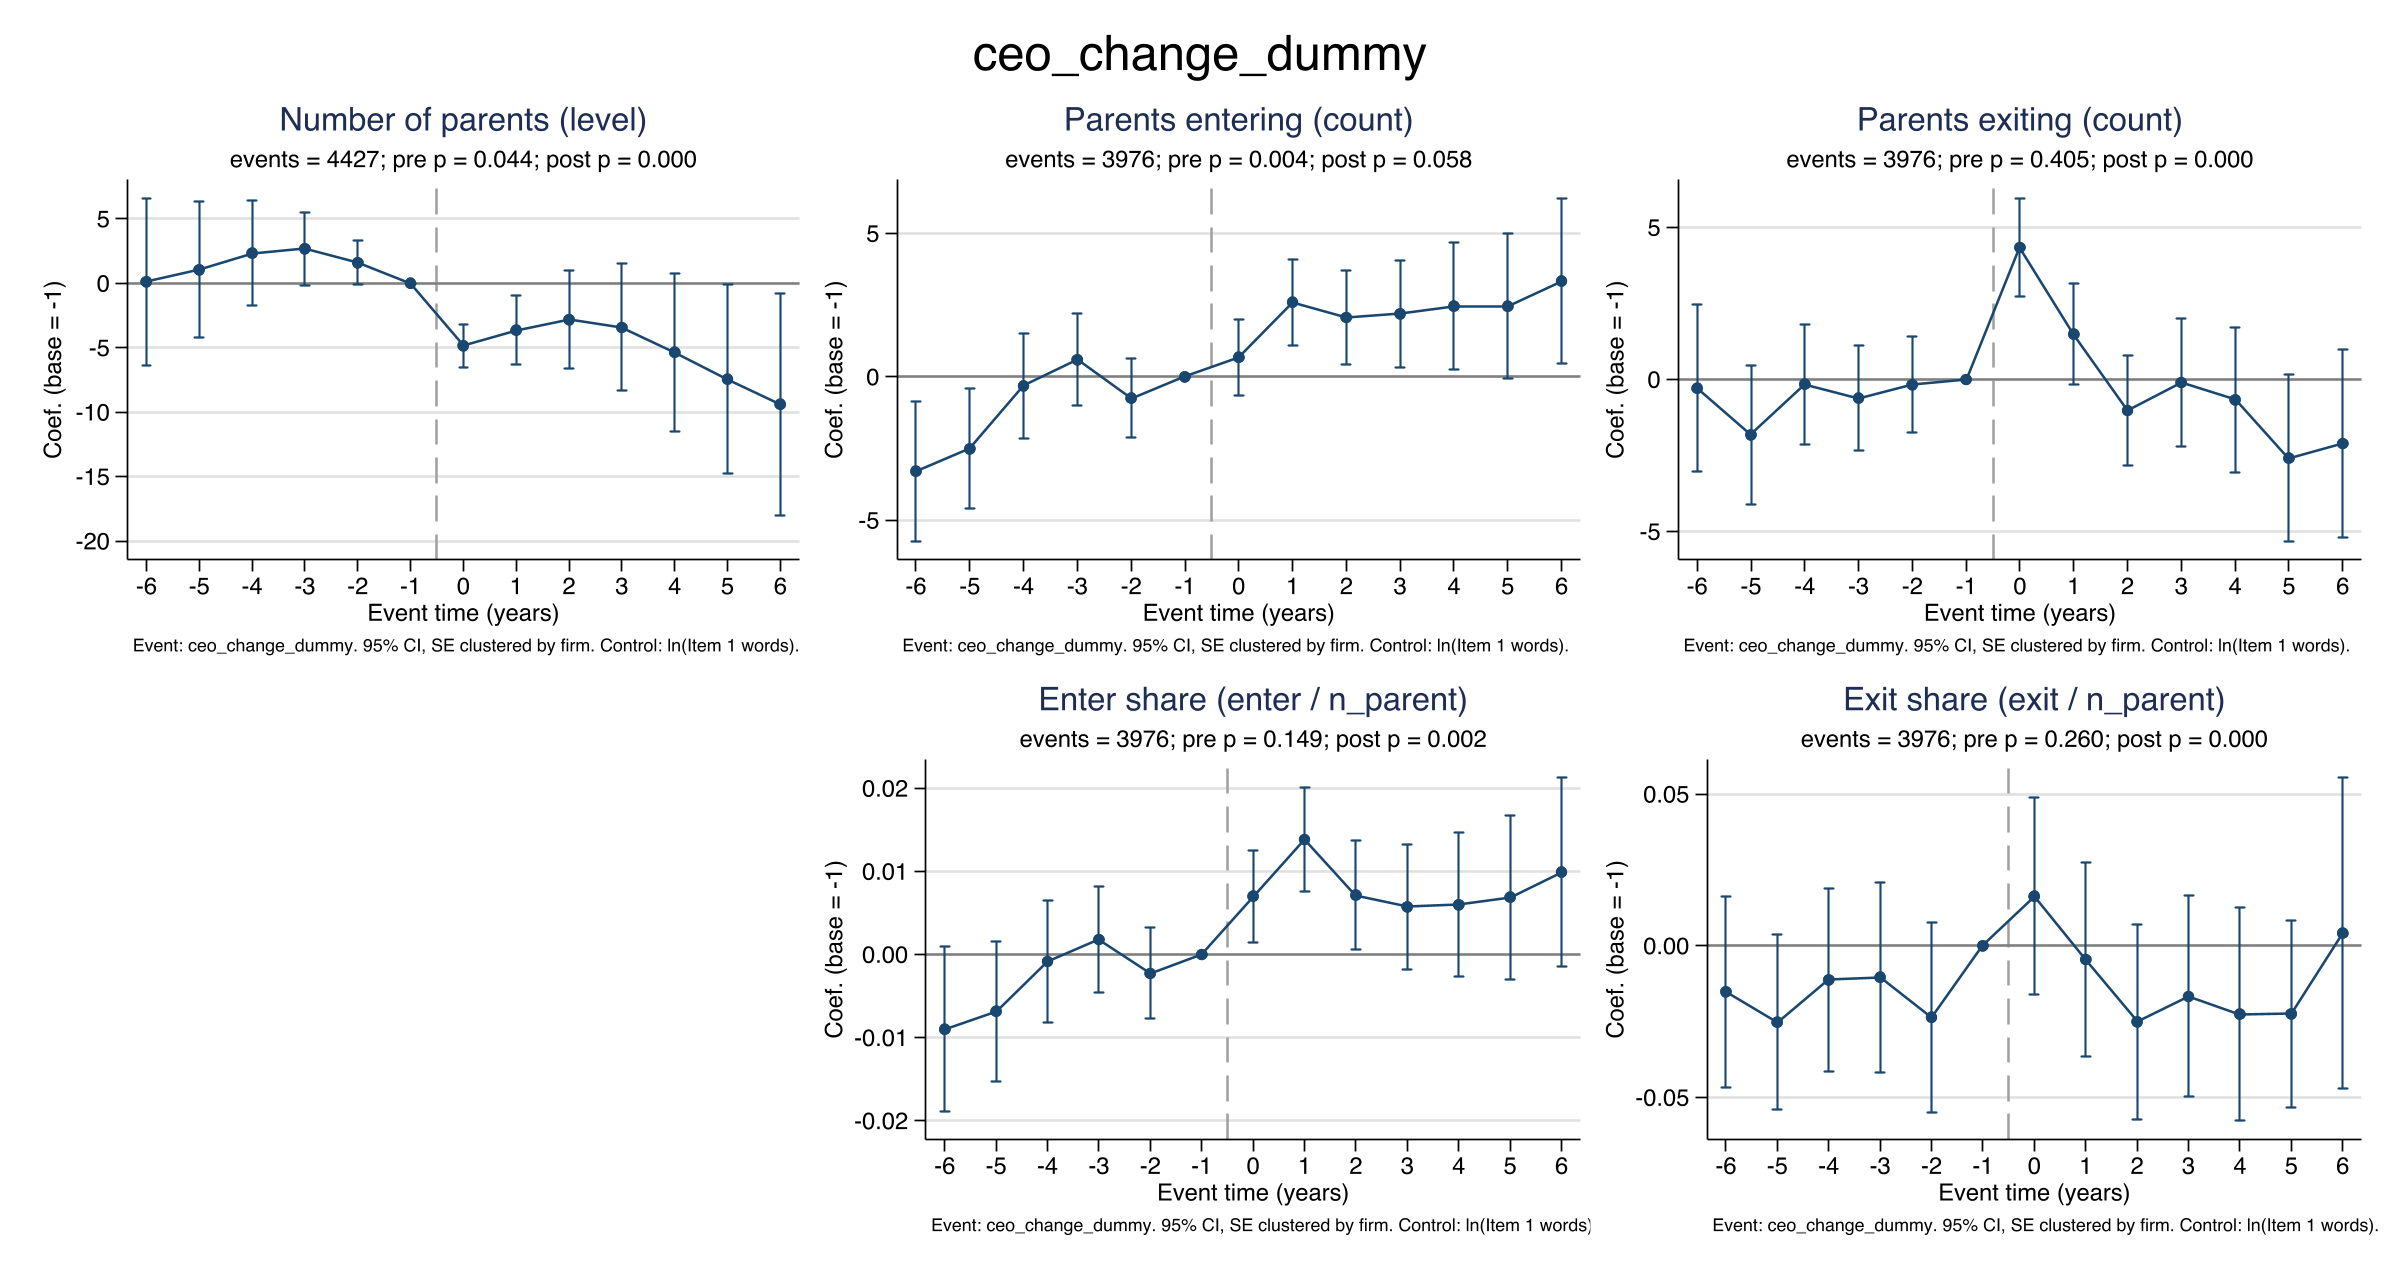
\includegraphics[width=\textwidth]{event_study/es_ceo_change_dummy_flows_combined.png}
\caption{Event study: CEO Change, with $\ln$(Item 1 words) control.}
\label{fig:es_ceo_change_dummy}
\end{figure}
\begin{figure}[H]
\centering
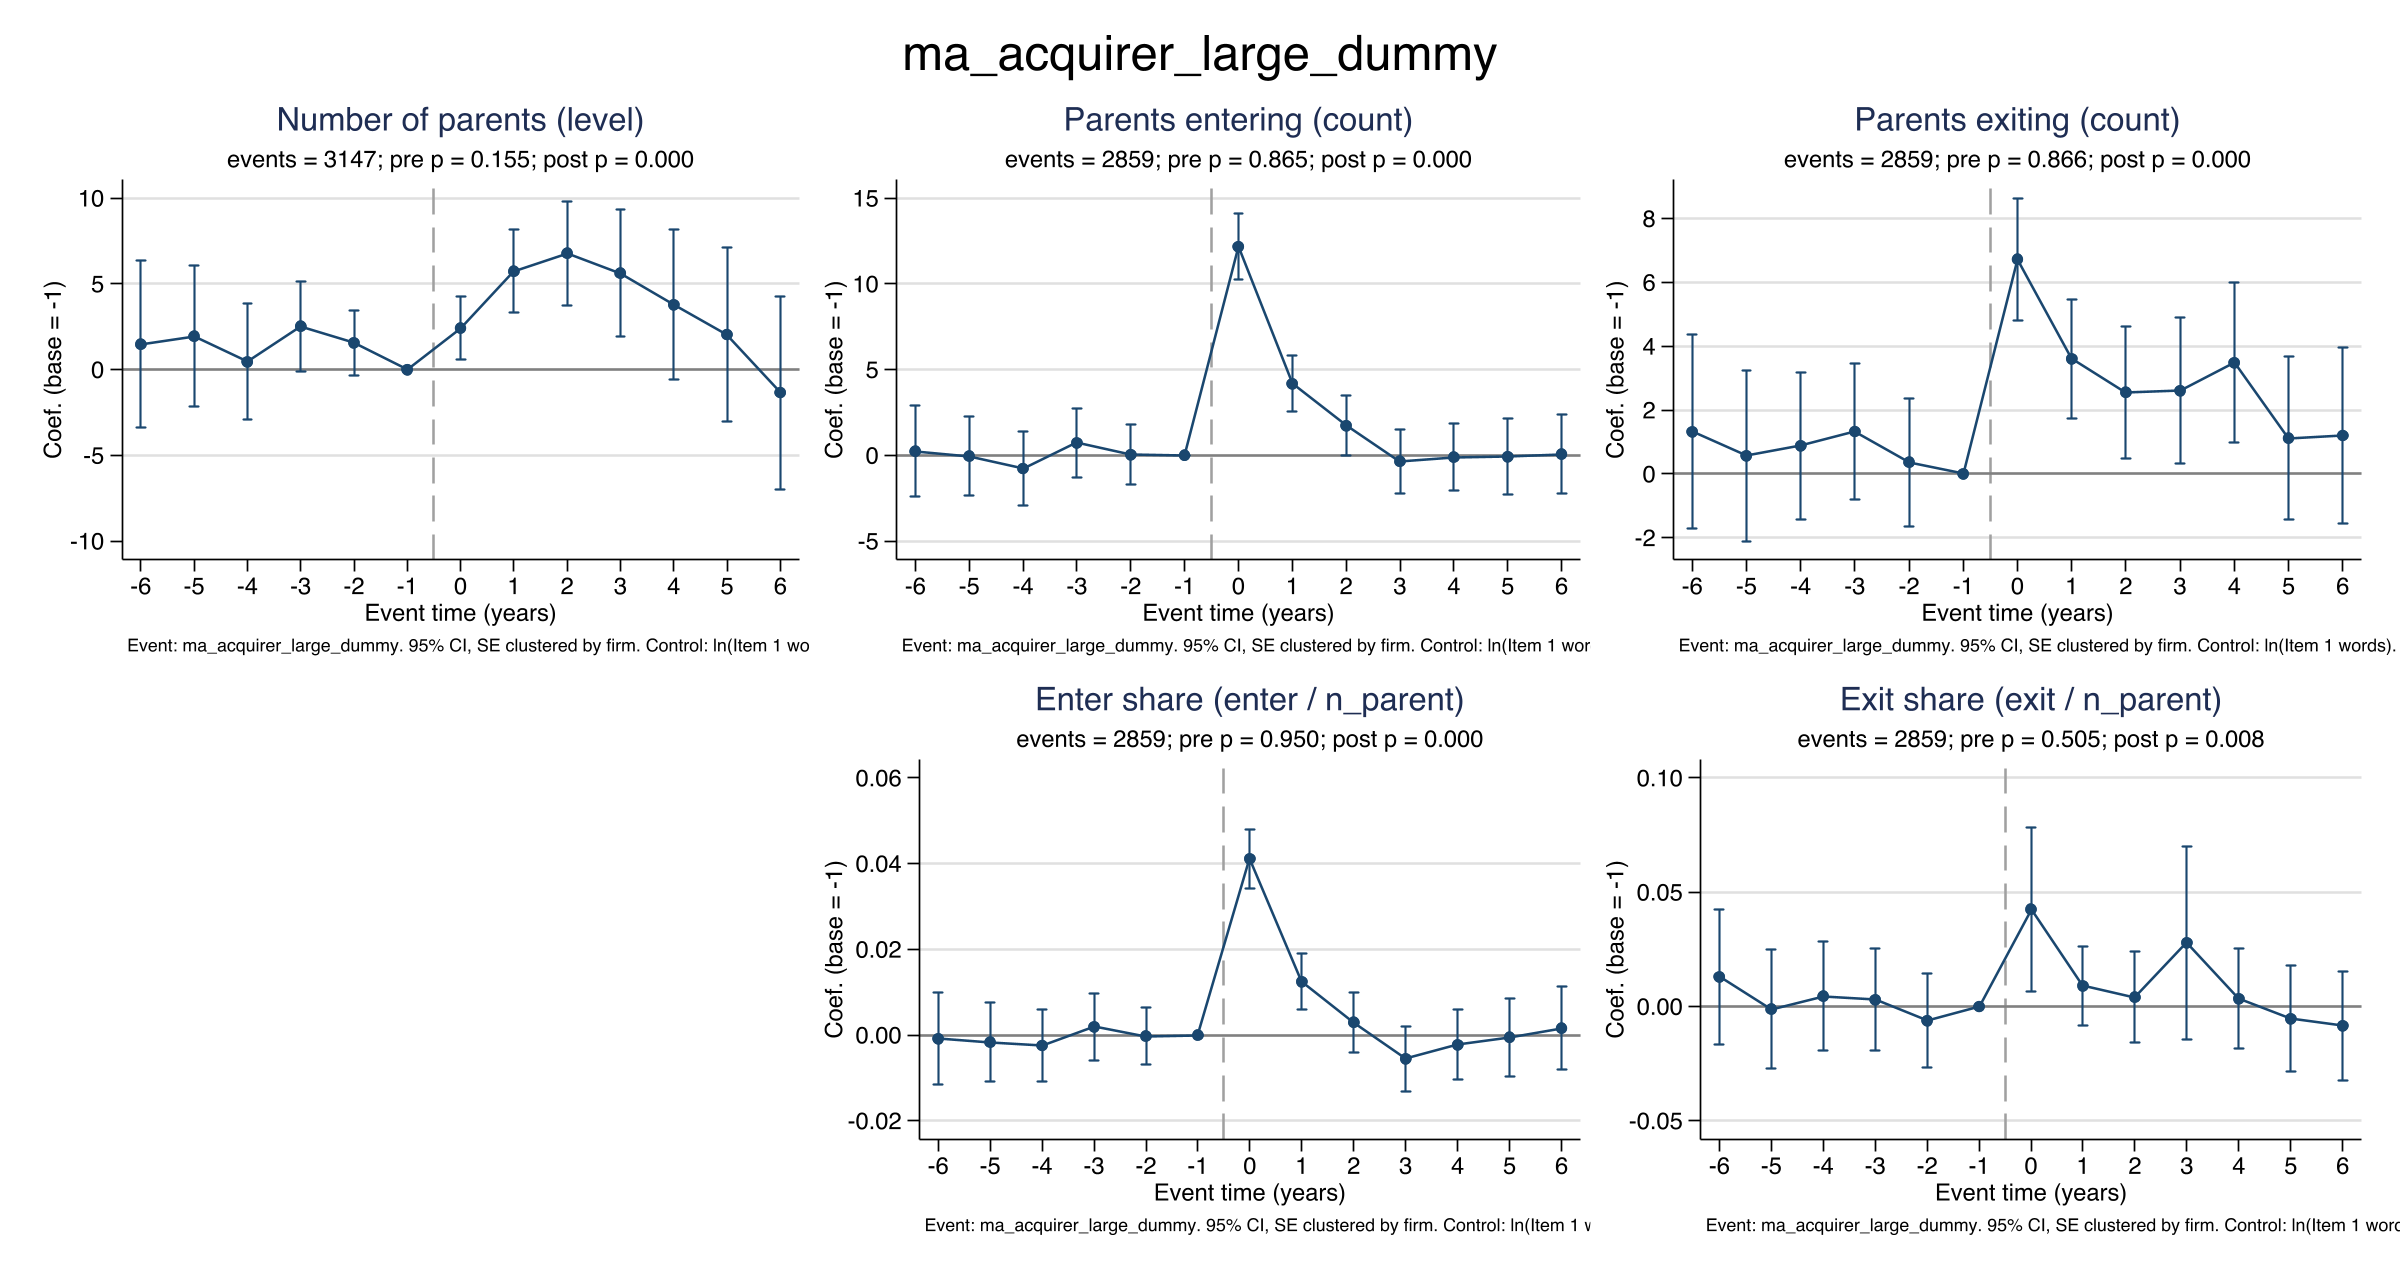
\includegraphics[width=\textwidth]{event_study/es_ma_acquirer_large_dummy_flows_combined.png}
\caption{Event study: Large M\&A Acquirer, with $\ln$(Item 1 words) control.}
\label{fig:es_ma_acquirer_large_dummy}
\end{figure}
\begin{figure}[H]
\centering
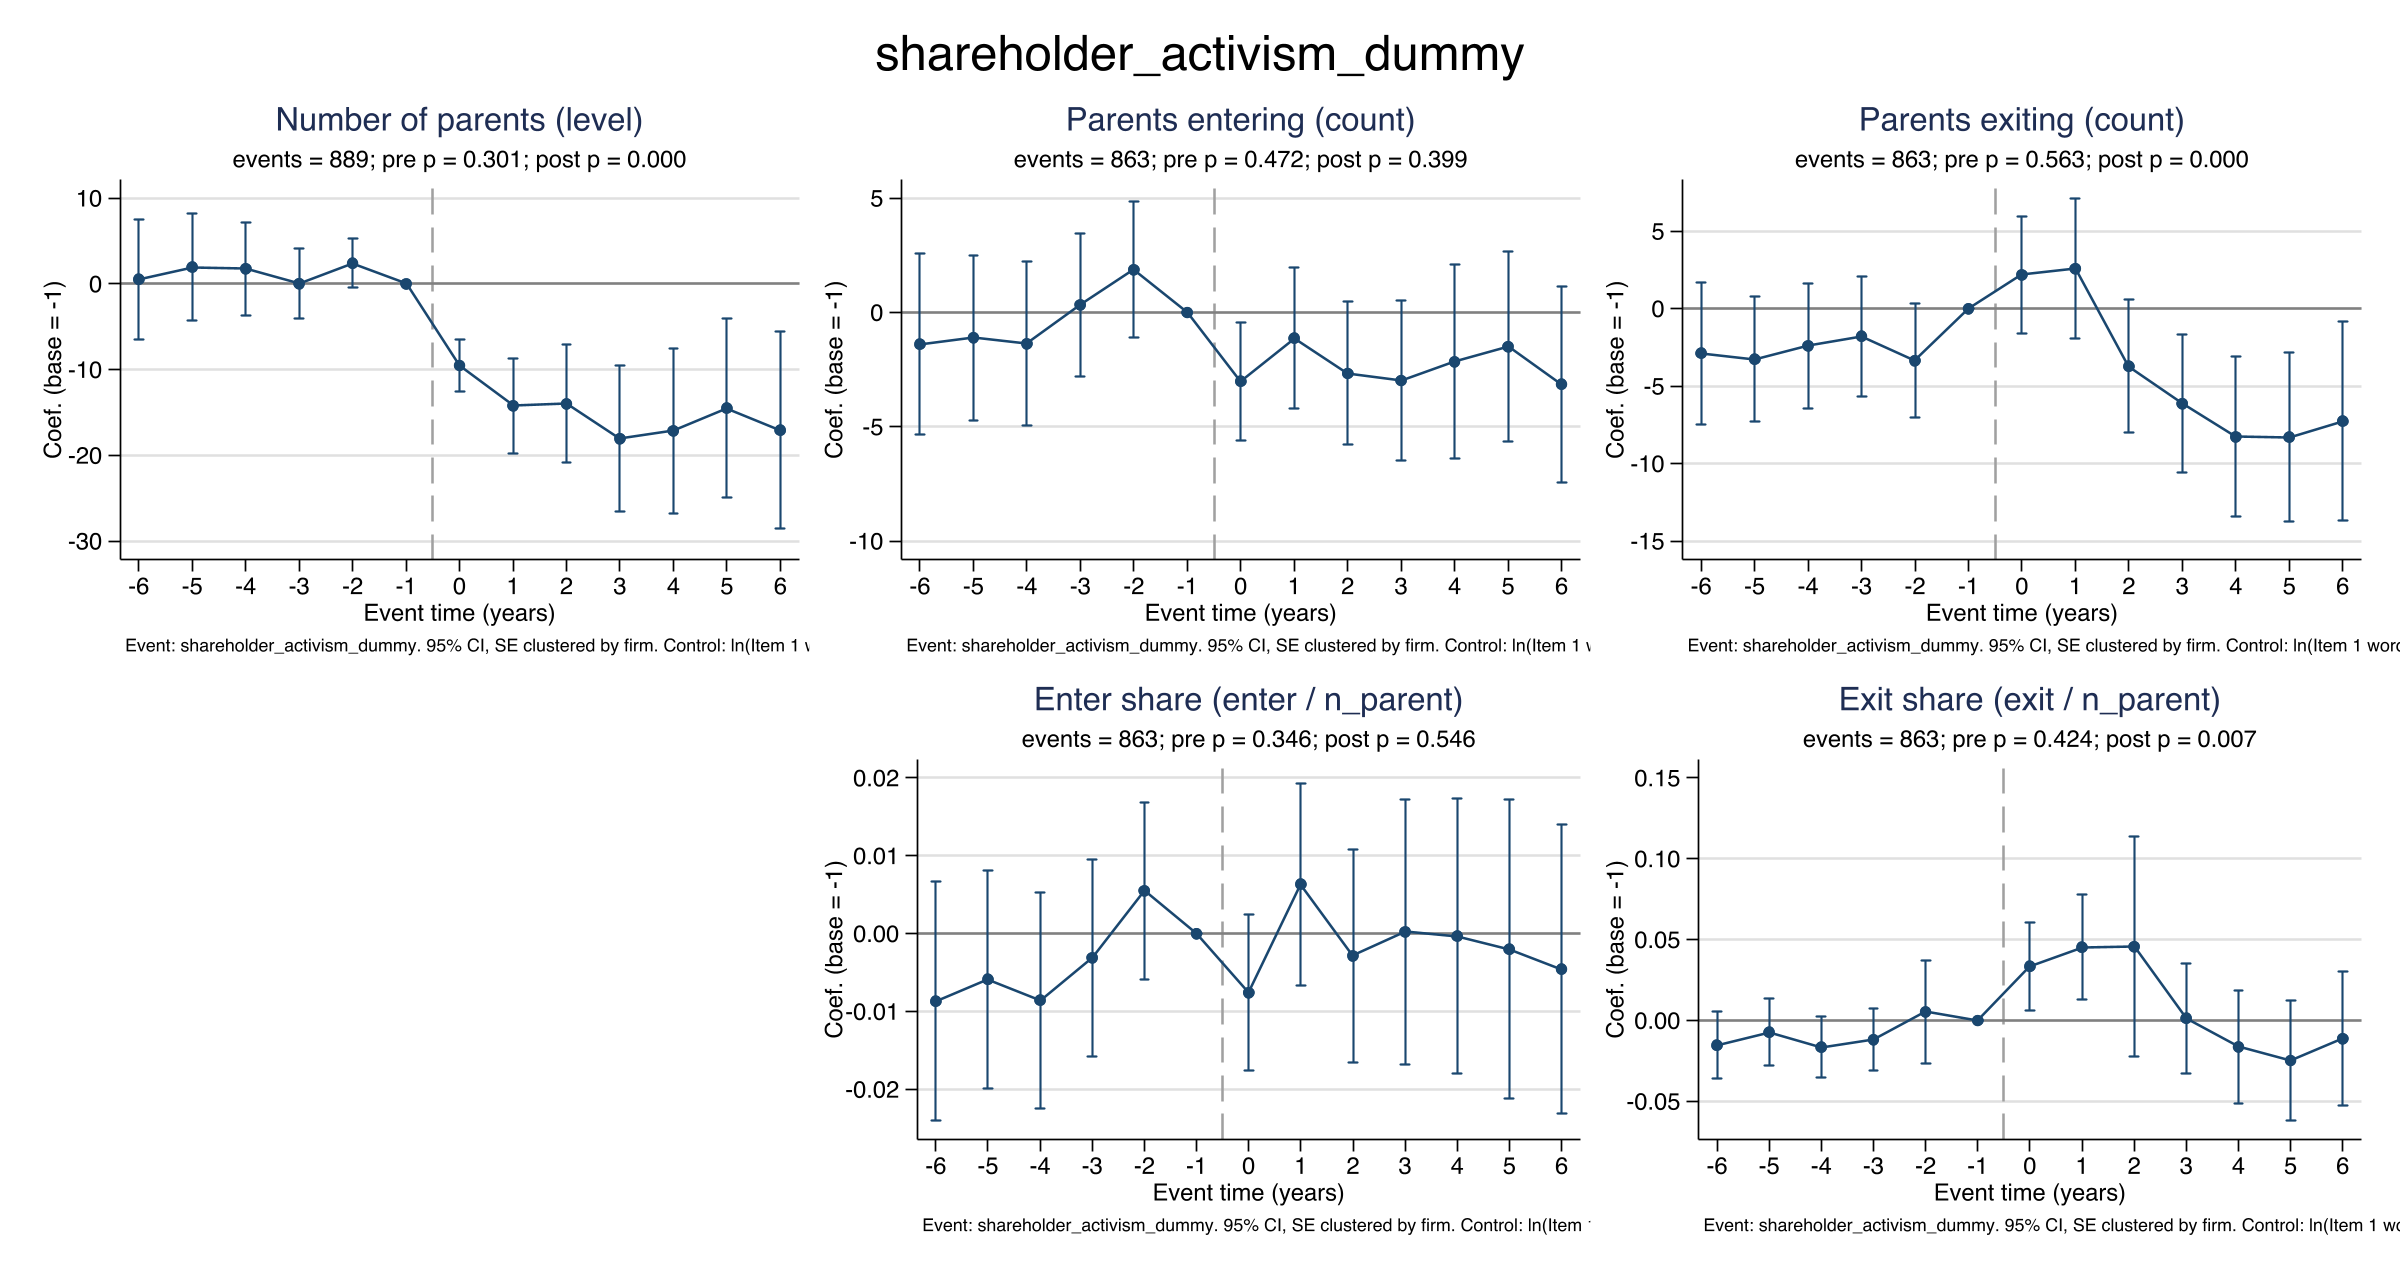
\includegraphics[width=\textwidth]{event_study/es_shareholder_activism_dummy_flows_combined.png}
\caption{Event study: Shareholder Activism, with $\ln$(Item 1 words) control.}
\label{fig:es_shareholder_activism_dummy}
\end{figure}
\begin{figure}[H]
\centering
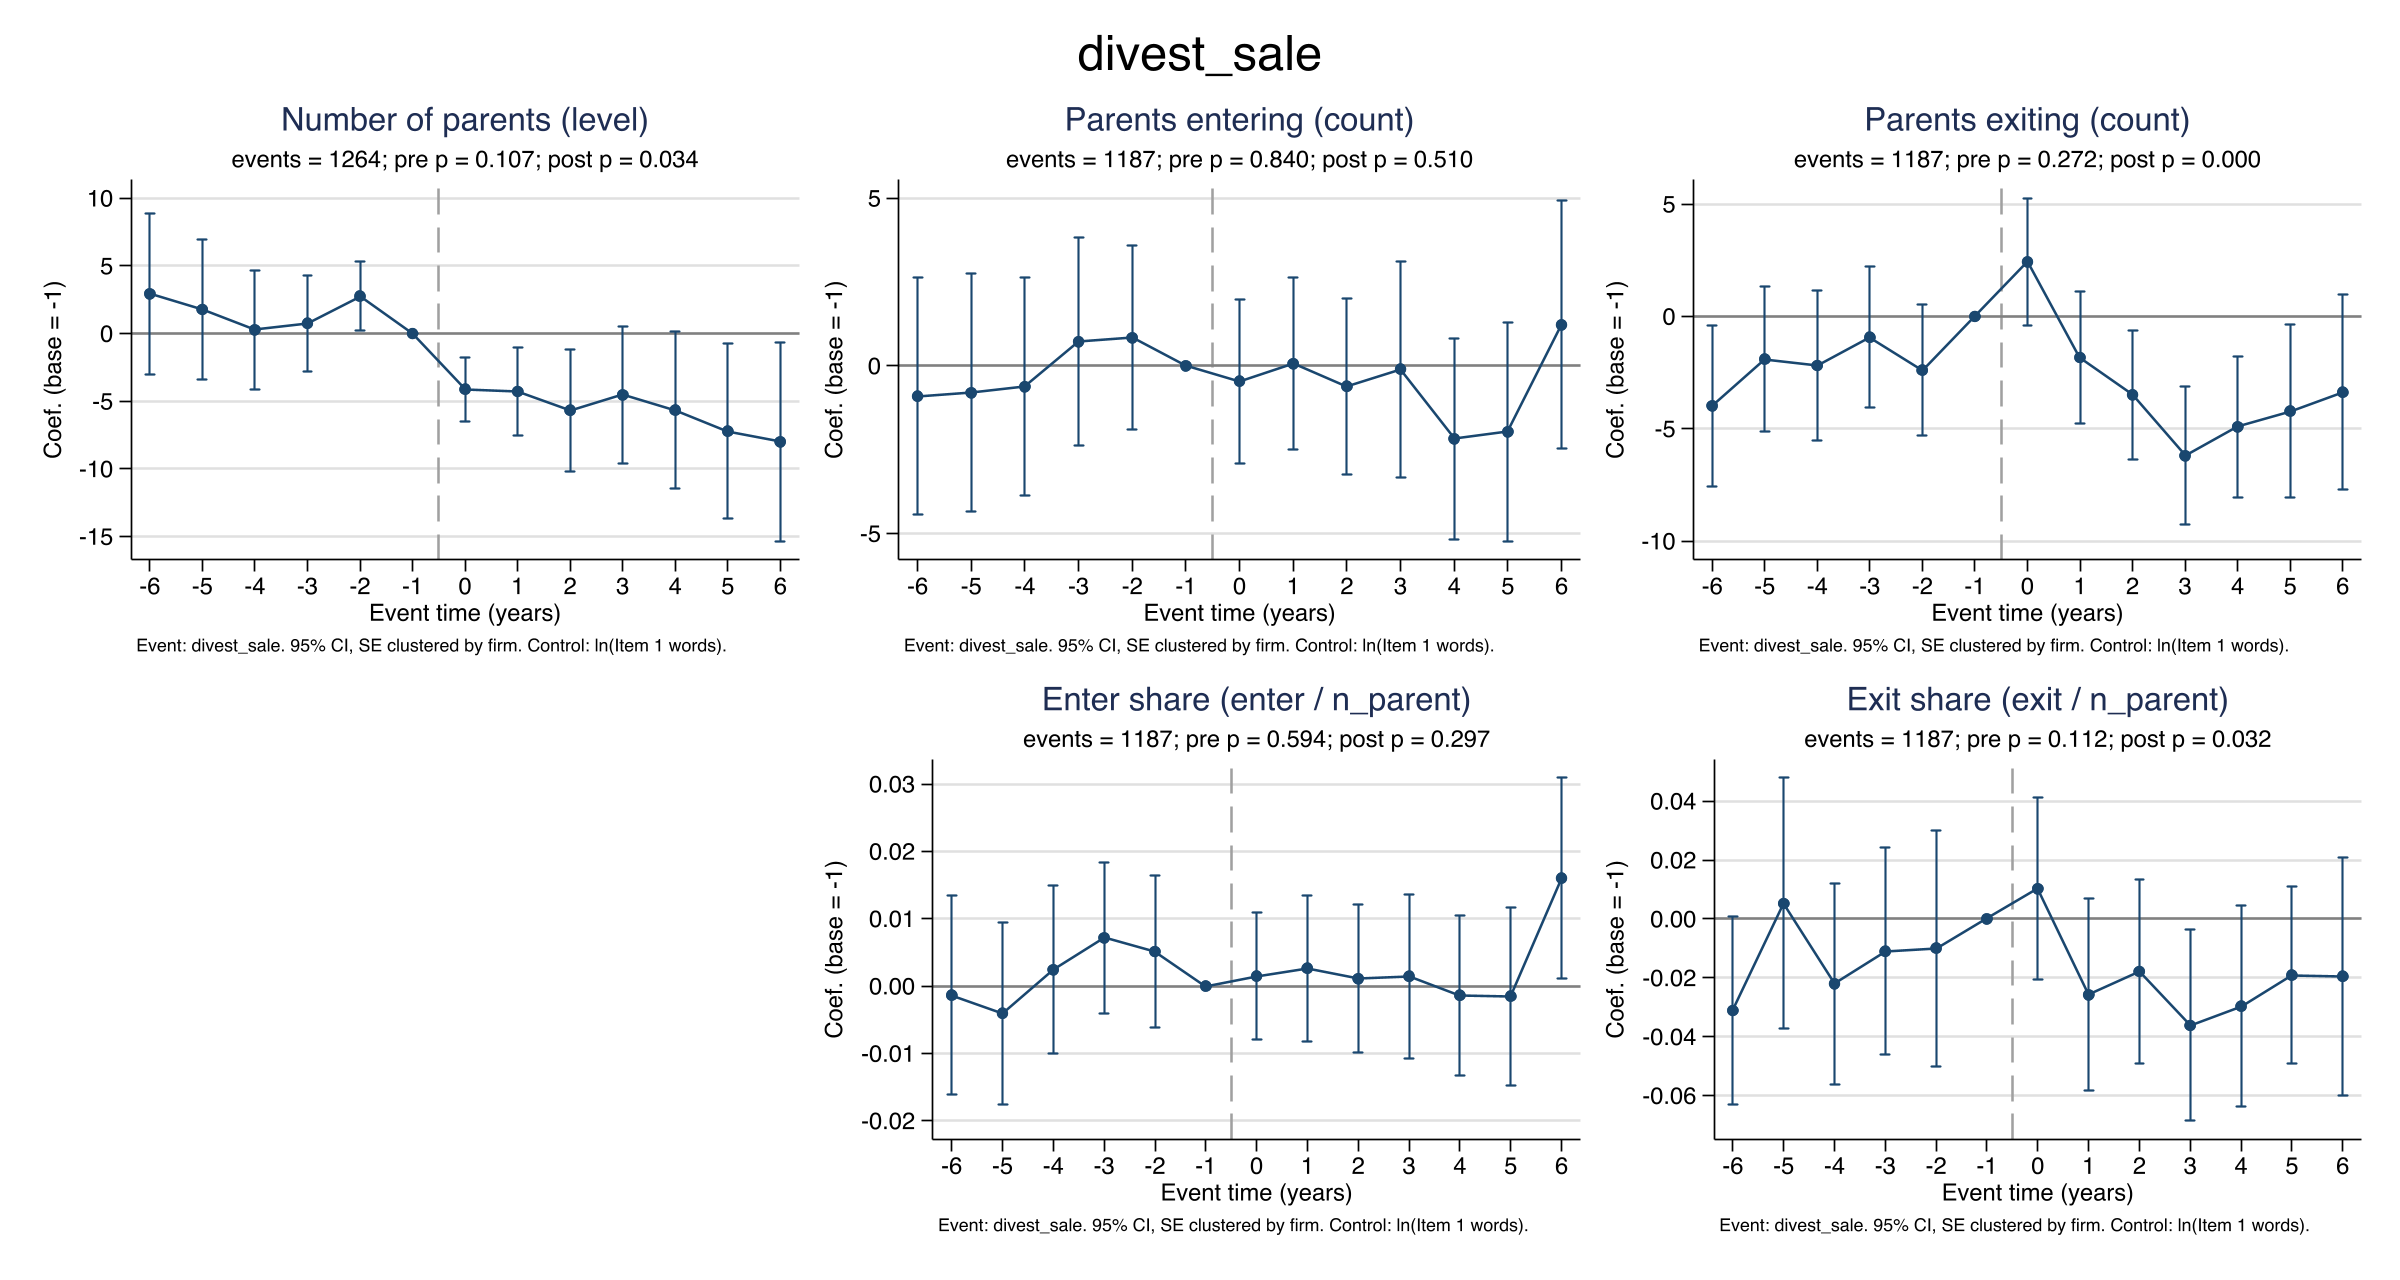
\includegraphics[width=\textwidth]{event_study/es_divest_sale_flows_combined.png}
\caption{Event study: Divestiture, with $\ln$(Item 1 words) control.}
\label{fig:es_divest_sale}
\end{figure}
\begin{figure}[H]
\centering
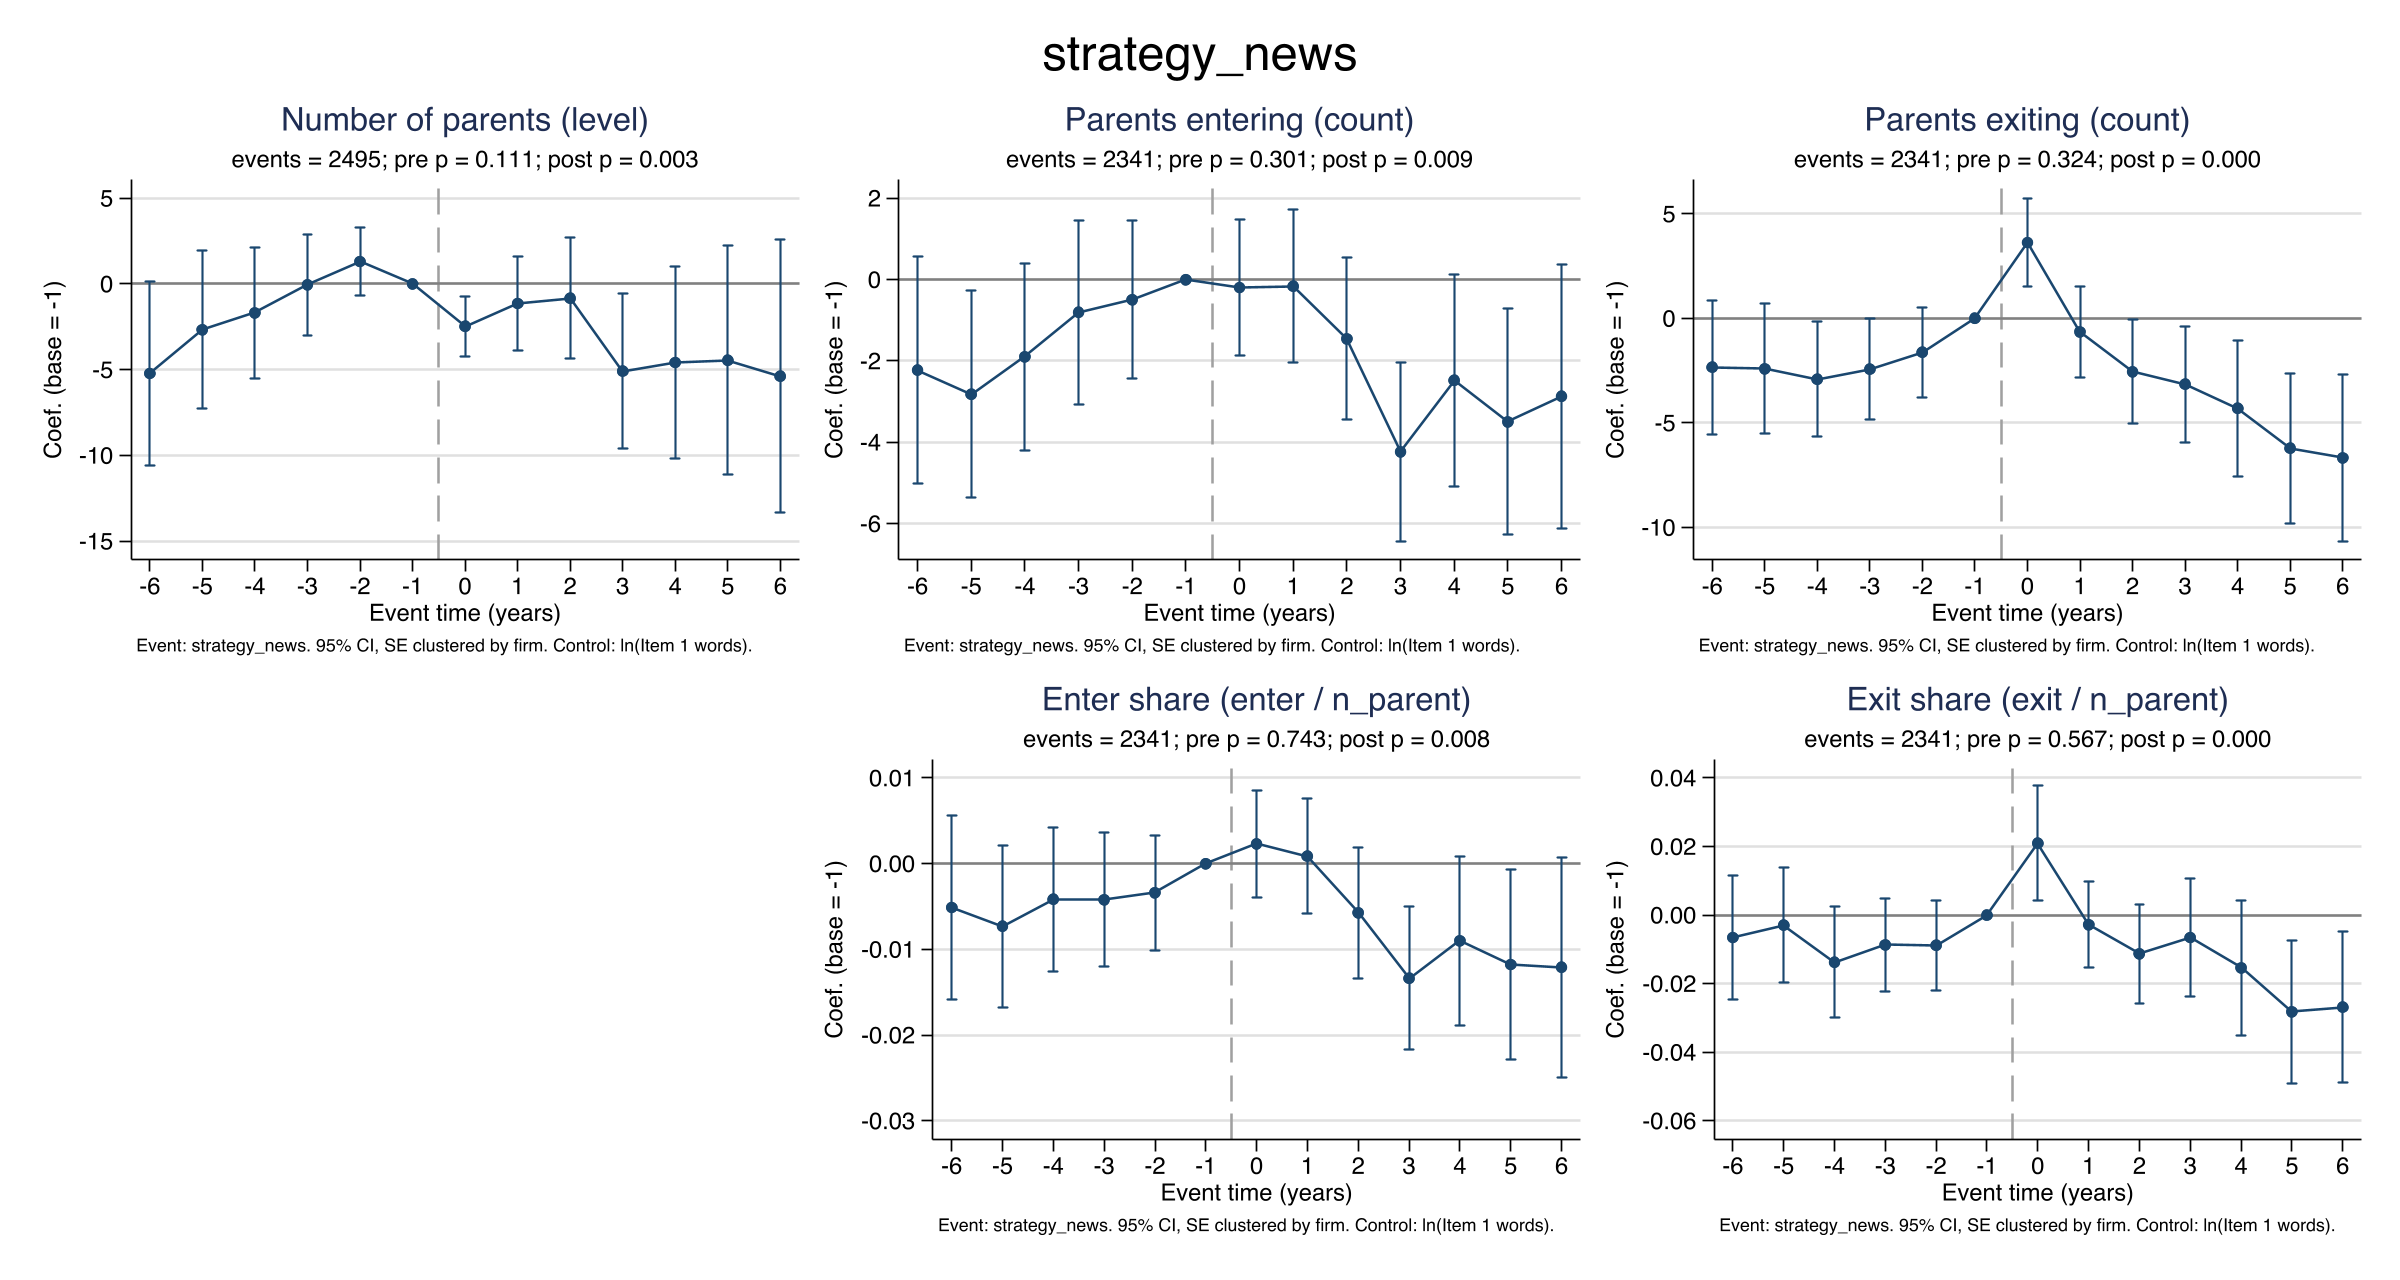
\includegraphics[width=\textwidth]{event_study/es_strategy_news_flows_combined.png}
\caption{Event study: Strategy News, with $\ln$(Item 1 words) control.}
\label{fig:es_strategy_news}
\end{figure}

\section{Uniqueness and Financial Performance}

Table~\ref{tab:dist_fin} relates financial ratios in year $t$ and $t+1$ to how far a firm's
business description lies from its closest peers in the same year. \texttt{dist\_top5} and
\texttt{dist\_top10} are the average embedding distances between the firm's Item 1 text and its
5 and 10 closest peers (larger values mean a more distinctive description). The regressions are plain
firm-year panel regressions (no stacking) with firm and year fixed effects and no other controls;
standard errors are clustered by firm.

\begin{landscape}
\begin{table}[H]
\centering
\caption{Uniqueness and Financial Performance}
\label{tab:dist_fin}
{\small Panel regressions with firm and year fixed effects}\\[4pt]
\begin{adjustbox}{max width=\linewidth, max totalheight=0.62\textheight}
\begin{tabular}{lcccccccccc}
\toprule
 & \multicolumn{2}{c}{ROA} & \multicolumn{2}{c}{ROIC} & \multicolumn{2}{c}{Operating margin} & \multicolumn{2}{c}{Net margin} & \multicolumn{2}{c}{Sales growth} \\
\cmidrule(lr){2-3} \cmidrule(lr){4-5} \cmidrule(lr){6-7} \cmidrule(lr){8-9} \cmidrule(lr){10-11}
 & $t$ & $t+1$ & $t$ & $t+1$ & $t$ & $t+1$ & $t$ & $t+1$ & $t$ & $t+1$ \\
 & (1) & (2) & (3) & (4) & (5) & (6) & (7) & (8) & (9) & (10) \\
\midrule
\multicolumn{11}{l}{\textit{Panel A. $x$ = Distance to 5 closest peers (\texttt{dist\_top5}); one SD $\approx$ 0.06}} \\[2pt]
Coefficient on $x$ & 0.0027 & 0.0438 & 0.0713 & 0.0619 & 0.0573 & 0.0911 & 0.0466 & 0.0849 & $-$0.0034 & 0.2054$^{**}$ \\
 & (0.0225) & (0.0227) & (0.0468) & (0.0494) & (0.0683) & (0.0778) & (0.0782) & (0.0880) & (0.0614) & (0.0639) \\
One-SD effect (pp) & 0.02 & 0.25 & 0.41 & 0.35 & 0.33 & 0.52 & 0.27 & 0.48 & $-$0.02 & 1.16 \\
Mean of $y$ (\%) & 3.40 & 3.52 & 18.55 & 18.47 & 10.21 & 10.63 & 1.21 & 1.70 & 13.59 & 12.38 \\
Observations & 40,394 & 37,296 & 32,223 & 29,851 & 40,280 & 37,184 & 40,283 & 37,184 & 40,205 & 37,150 \\
Firms & 2,403 & 2,309 & 2,177 & 2,089 & 2,400 & 2,306 & 2,401 & 2,306 & 2,397 & 2,304 \\
Within $R^2$ & 0.0000 & 0.0003 & 0.0002 & 0.0001 & 0.0001 & 0.0001 & 0.0000 & 0.0001 & 0.0000 & 0.0005 \\
\cmidrule(l){1-11}
\addlinespace[4pt]
\multicolumn{11}{l}{\textit{Panel B. $x$ = Distance to 10 closest peers (\texttt{dist\_top10}); one SD $\approx$ 0.06}} \\[2pt]
Coefficient on $x$ & 0.0104 & 0.0525$^{*}$ & 0.0869 & 0.0803 & 0.0706 & 0.1045 & 0.0595 & 0.0915 & 0.0189 & 0.2430$^{***}$ \\
 & (0.0219) & (0.0224) & (0.0460) & (0.0481) & (0.0690) & (0.0782) & (0.0780) & (0.0878) & (0.0611) & (0.0646) \\
One-SD effect (pp) & 0.06 & 0.32 & 0.53 & 0.48 & 0.43 & 0.63 & 0.36 & 0.55 & 0.11 & 1.46 \\
Mean of $y$ (\%) & 3.40 & 3.52 & 18.55 & 18.47 & 10.21 & 10.63 & 1.21 & 1.70 & 13.59 & 12.38 \\
Observations & 40,394 & 37,296 & 32,223 & 29,851 & 40,280 & 37,184 & 40,283 & 37,184 & 40,205 & 37,150 \\
Firms & 2,403 & 2,309 & 2,177 & 2,089 & 2,400 & 2,306 & 2,401 & 2,306 & 2,397 & 2,304 \\
Within $R^2$ & 0.0000 & 0.0004 & 0.0003 & 0.0002 & 0.0001 & 0.0002 & 0.0000 & 0.0001 & 0.0000 & 0.0008 \\
\midrule
Firm fixed effects & Yes & Yes & Yes & Yes & Yes & Yes & Yes & Yes & Yes & Yes \\
Year fixed effects & Yes & Yes & Yes & Yes & Yes & Yes & Yes & Yes & Yes & Yes \\
\bottomrule
\end{tabular}
\end{adjustbox}
\\[4pt]
\begin{minipage}{\linewidth}\footnotesize
\textit{Notes.} Each cell is a separate regression of the financial ratio in year $t$ or $t+1$ on a peer-distance measure in year $t$, with firm and year fixed effects and no other controls. Coefficients are raw (ratios in decimals; 0.01 = 1\%). Standard errors clustered by firm are in parentheses. One-SD effect is the coefficient times the standard deviation of the distance measure in the estimation sample, in percentage points of the ratio. Financial ratios are winsorized at the pooled 1st and 99th percentiles; $t+1$ outcomes are missing when year $t+1$ is not observed. $^{*}p<0.05$, $^{**}p<0.01$, $^{***}p<0.001$.
\end{minipage}
\end{table}
\end{landscape}

\end{document}
